\documentclass[11pt,letterpaper]{article}

\usepackage[spanish,es-tabla,es-nodecimaldot]{babel}
\usepackage{amsmath}
\usepackage[utf8]{inputenc}
\usepackage[T1]{fontenc}
\usepackage{lmodern}
\usepackage{graphicx}
\usepackage{listings}
\usepackage{anysize} 
\usepackage{fancyhdr}
\usepackage{amsmath}
\usepackage{pdfpages}
\usepackage{graphics}
\usepackage{capt-of}
\usepackage{tabularx}
\usepackage{rotating}
\usepackage{tikz}
\usepackage[colorlinks=true,plainpages=true,citecolor=blue,linkcolor=blue]{hyperref}

\usepackage{xcolor}
\definecolor{mGreen}{rgb}{0,0.6,0}
\definecolor{mGray}{rgb}{0.5,0.5,0.5}
\definecolor{mPurple}{rgb}{0.58,0,0.82}
\definecolor{backgroundColour}{rgb}{0.95,0.95,0.92}

\marginsize{2cm}{2cm}{2cm}{2cm}
\pagestyle{fancy}
\fancyhf{Sistemas celulares}
\fancyhead[L]{\footnotesize UPIITA-IPN} 
\fancyhead[R]{\footnotesize 2TV7} 
\fancyfoot[R]{\footnotesize Tarea 2}
\fancyfoot[C]{\thepage}
\fancyfoot[L]{\footnotesize } 

\renewcommand{\footrulewidth}{0.4pt}
\renewcommand{\spanishtablename}{Tabla}
\renewcommand{\labelitemii}{$\star$}

\lstdefinestyle{CStyle}{
    backgroundcolor=\color{backgroundColour},   
    commentstyle=\color{mGreen},
    keywordstyle=\color{magenta},
    numberstyle=\tiny\color{mGray},
    stringstyle=\color{mPurple},
    basicstyle=\footnotesize,
    breakatwhitespace=false,         
    breaklines=true,                 
    captionpos=b,                    
    keepspaces=true,                 
    numbers=left,                    
    numbersep=5pt,                  
    showspaces=false,                
    showstringspaces=false,
    showtabs=false,                  
    tabsize=2,
    language=C
}

\graphicspath{ {C:/Users/Anselmo/Documents/GitHub/upiita-SistemasCelulares/Tarea2c/imagenes} }

\begin{document}

\includepdf[pages={1}]{Portada}

\newpage
\tableofcontents
\listoffigures
\listoftables

\newpage
\section{Conetxto}
El siguiente análisis tiene por objetivo diseñar una red celular bajo el marco de trabajo AMPS 
que cubra el municipio de Nezahualcóyotl que fue el área de estudio del trabajo anterior. 
Advanced Mobile Phone Service (AMPS) es un sistema estándar para el servicio de telefonía 
celular con señal analógica. 
\\ \\
AMPS asigna rangos de frecuencia dentro del espectro de 800 y 900 Megahertz (MHz) al teléfono 
celular. Cada proveedor de servicios puede utilizar la mitad de la gama de 824-849 MHz para 
recibir señales de teléfonos celulares y la mitad de la gama de 869-894 MHz para transmitir 
a teléfonos celulares. Las bandas se dividen en sub-bandas de 30 kHz, llamadas canales. Los 
canales de recepción se denominan canales inversos y los canales de envío se denominan 
canales de avance. La división del espectro en canales de sub-banda se consigue utilizando 
el acceso múltiple por división de frecuencia (FDMA).
\\ \\
Las señales recibidas de un transmisor cubren un área llamada célula. A medida que un usuario 
se mueve fuera del área de la célula hacia una célula adyacente, el usuario comienza a 
captar las señales de la nueva célula sin ninguna transición notable. Las señales en la 
célula adyacente son enviadas y recibidas en canales diferentes a las señales de la célula 
anterior para que las señales no interfieran entre sí.
\\ \\
A continuación se presenta un diagrama general del concepto.
\begin{figure}[ht]
    \centering
    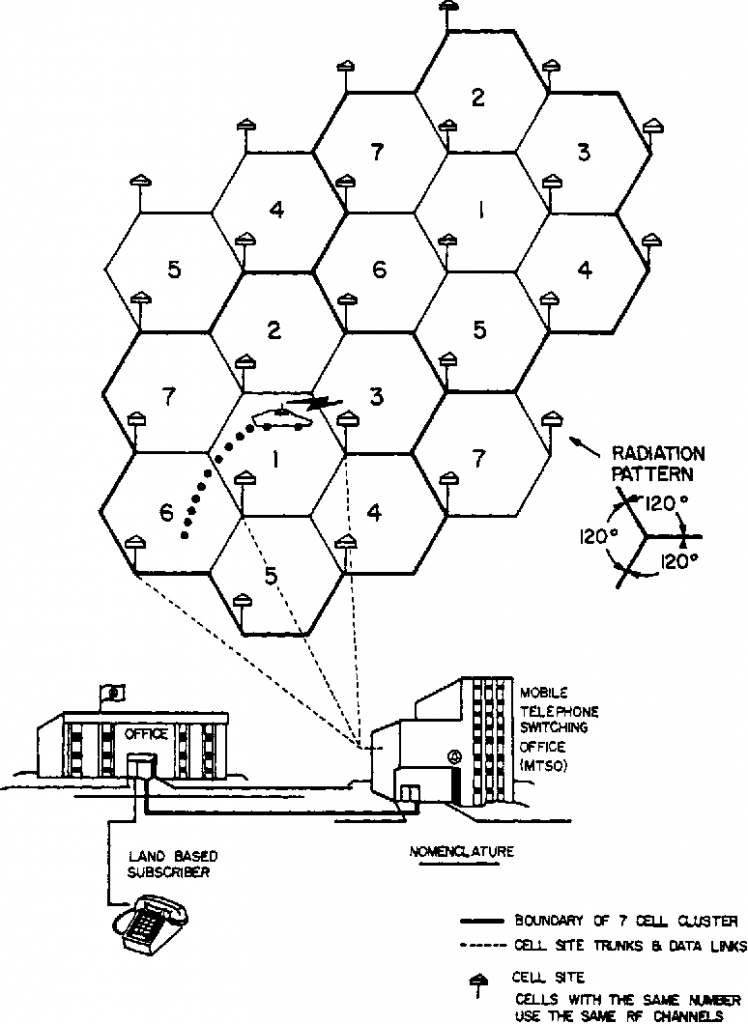
\includegraphics[width=0.45\textwidth]{imagenes/t20.png}
    \caption{AMPS.}
\end{figure}
\\
Las condiciones iniciales del estudio parten de la época de los 80s, que fue cuando AMPS fue 
introducido a México. Es así como se propone que el estimado de población usuaria de un 
dispositivo móvil presente en la región sea del 5\% de la población actual. De acuerdo con 
información publicada por el INEGI, la población actual del municipio es de 1,228,654 
habitantes. Este supuesto nos deja con una población usuaria de un dispositivo celular sea 
de 61432.7 personas. Otra condición importante para señalar es el de evitar radiar las zonas 
de escuelas, hospitales, parques, cemneterios y zonas inhabitadas, por mecionar algunas. 
\begin{figure}[ht]
    \centering
    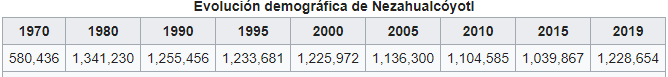
\includegraphics[width=0.9\textwidth]{imagenes/t21.png}
    \caption{Evolución demográfica.}
\end{figure}

\section{Análisis}
Como se mencionó en la sección anterior hay zonas que no se busca que sean radiadas. Estas 
áreas se mostrarán sombreadas dentro del mapa que se anexará al estudio. Otro dato importante 
que debe obtenerse es el área del patrón de radiación que tendrá la antena.  

\subsection{Área del patrón de radiación}
Teniendo como referencia la siguiente imagen, se obtiene el área del cardiode.
\begin{figure}[ht]
    \centering
    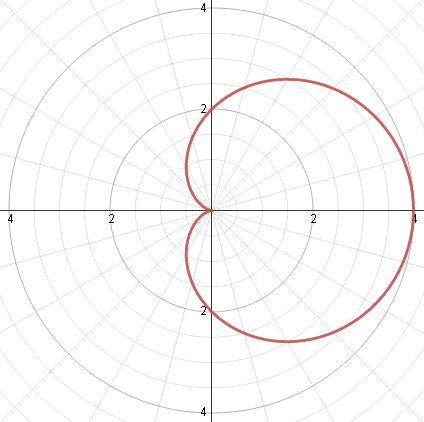
\includegraphics[width=0.4\textwidth]{imagenes/t22.jpg}
    \caption{Cardiode.}
\end{figure}
\\
Partiendo de la siguiente expresión.
\begin{equation}
    A=\int_{0}^{\pi} \rho^2 d\theta = \frac{3}{2} a^2 \pi
\end{equation}
Y resolviendo para $a$.
\begin{equation}
    a^2=\frac{2(1km^2)}{3\pi}=212.2 \ m^2
\end{equation}
Es así como el área del cardiode cubre un área de $212.2 \ m^2$.

\subsection{Niveles de comunicación}
Tomando como referencia los niveles de recepción vistos en clase, se proponen los 
siguientes intervalos para el estudio. 
\begin{table}[ht]
    \centering
    \begin{tabular}{|l|l|}
    \hline
    $P_{Rx}$ [dB] & Niveles de comunicación \\ \hline
    [0, -40] & Comunicación buena \\ \hline
    [-41, -70] & Comunicación normal \\ \hline
    [-71, -90] & Alta posibilidad de perdida de comunicación \\ \hline
    \end{tabular}
    \caption{Niveles de recepción.}
\end{table}
\\
Lo que se pretende es ofrecer un servicio normal de comunicación, por lo que el 
siguiente paso es encontrar la distancia, la cual permitirá una comunicación normal, 
es decir, que la potencia de recepción ($P_{Rx}$) tenga un valor aproximado a -70dB.
\\ \\
Partiendo de los datos del estudio anterior.
\\ \\
Datos del estudio anterior.
\begin{itemize}
    \item hb: 19m.
    \item hm: 1.7m.
    \item d: 462.94m.
    \item f: 900 MHz.
    \item $L_o$=84.817 dB.
    \item $P_{Tx}$: 0.1 W.
    \item $G_{Rx}$: 4.6 dB.
    \item $G_{Tx}$: 14.56 dB.
    \item $P_{Rx}$: -57.46 dBm.
\end{itemize}

Y de la siguientes expresiones.
\begin{equation}
    L_o=32.44+20\log{fMHz}+20\log{dKm}
\end{equation}
\begin{equation}
    P_{Rx}=(\frac{hb*hm}{d^2})^2 (\frac{G_{Tx}*G_{Rx}}{L_0}) P_{Tx}
\end{equation}

\newpage
Resolviendo para $d$ y tomando de referencia el estudio anterior se obtiene que la distancia 
a la cual el nivel de comunicación está en el límite de la potencia de recepción de -70dB es 
de 936.5 metros.
\begin{equation}
    L_o=32.44+20\log{900MHz}+20\log{0.9365 Km}=90.915 \ dB
\end{equation}
\begin{equation}
    P_{Rx}=(\frac{19*1.7}{936.5^2})^2 (\frac{14.56*4.6}{L_0}) 0.1=9.992x10^{-11} W
\end{equation}
\begin{equation}
    P_{Rx}=10\log{\frac{P_{Rx}}{0.001}}=-70dB
\end{equation}

\subsection{Establecimiento de células}
Se tomará como punto de referencia el ayuntamiento del municipio, el cual puede considerarse 
una zona de interés la cual debe contar con un buen servicio de comunicación. A partir de 
ahí, se colocarán las células tomando en cuenta la áreas que no deben radiarse.
\\ \\ 
Se presenta una tabla donde se exponen los parámetros usados en la expresión número 6, con 
su respectiva potencia de recepción. La rutina usada para calcular las potencias de 
recepción se muestra en el anexo de este estudio. 

\newpage
\begin{table}[ht]
    \centering
    \begin{tabular}{|l|l|l|l|l|l|l|l|l|l|l|l|l|l|l|}
    \hline
    Clúster & Célula & Sector & hb[m] & d[m] & $G_{Tx}$[dB] & $G_{Rx}$[dB] & $L_o[dB]$ & $P_{Rx}[dB]]$ \\ \hline
    1 & 1 & 1 & 21 & 936.5 & 14.56 & 4.6 & 90.92 & -69.13 \\ \hline
    1 & 1 & 2 & 20 & 930 & 14.56 & 4.6 & 90.85 & -69.43 \\ \hline
    1 & 1 & 3 & 20 & 950 & 14.56 & 4.6 & 91.04 & -69.81 \\ \hline
    1 & 2 & 1 & 19 & 930 & 14.56 & 4.6 & 90.85 & -69.88 \\ \hline
    1 & 2 & 2 & 19.5 & 940 & 14.56 & 4.6 & 90.95 & -69.84 \\ \hline
    1 & 2 & 3 & 20 & 938 & 14.56 & 4.6 & 90.93 & -69.59 \\ \hline
    1 & 3 & 1 & 22 & 935 & 14.56 & 4.6 & 90.9 & -68.7 \\ \hline
    1 & 4 & 1 & 22 & 920 & 14.56 & 4.6 & 90.76 & -68.41 \\ \hline
    1 & 5 & 1 & 20 & 936 & 14.56 & 4.6 & 90.91 & -69.55 \\ \hline
    1 & 5 & 2 & 19 & 938 & 14.56 & 4.6 & 90.93 & -70.03 \\ \hline
    1 & 6 & 1 & 19 & 940 & 14.56 & 4.6 & 90.95 & -70.07 \\ \hline
    1 & 6 & 2 & 19.5 & 933 & 14.56 & 4.6 & 90.88 & -69.71 \\ \hline
    1 & 7 & 1 & 21 & 930 & 14.56 & 4.6 & 90.85 & -69.01 \\ \hline
    1 & 7 & 2 & 20 & 935 & 14.56 & 4.6 & 90.9 & -69.53 \\ \hline
    2 & 1 & 1 & 19 & 937 & 14.56 & 4.6 & 90.92 & -70.01 \\ \hline
    2 & 1 & 2 & 20 & 936 & 14.56 & 4.6 & 90.91 & -69.55 \\ \hline
    2 & 1 & 3 & 22 & 938 & 14.56 & 4.6 & 90.93 & -68.76 \\ \hline
    2 & 2 & 1 & 24 & 940 & 14.56 & 4.6 & 90.95 & -68.04 \\ \hline
    2 & 3 & 1 & 25 & 936 & 14.56 & 4.6 & 90.91 & -67.61 \\ \hline
    2 & 3 & 2 & 22 & 942 & 14.56 & 4.6 & 90.97 & -68.83 \\ \hline
    2 & 3 & 3 & 21 & 950 & 14.56 & 4.6 & 91.04 & -69.39 \\ \hline
    2 & 4 & 1 & 19 & 937 & 14.56 & 4.6 & 90.92 & -70.01 \\ \hline
    2 & 4 & 2 & 19.5 & 938 & 14.56 & 4.6 & 90.93 & -69.81 \\ \hline
    2 & 5 & 1 & 26 & 937 & 14.56 & 4.6 & 90.92 & -67.29 \\ \hline
    2 & 5 & 2 & 25 & 936.5 & 14.56 & 4.6 & 90.92 & -67.62 \\ \hline
    2 & 6 & 1 & 20 & 940 & 14.56 & 4.6 & 90.95 & -69.62 \\ \hline
    \end{tabular}
    \caption{Estudio.}
\end{table}

\newpage
\section{Análisis y asignación de frecuencias}
Una vez establecidas las células, sigue la asignación y reutilización de frecuencias. 
Esta tarea se realizará con el método [i, j], estudiado en clase. Se tomará como base 
un clúster formado por 7 células. Así, los valores que tomaran i y j son 1 y 2 
respectivamente. La siguiente imagen muestra la tabla en la cual se basa esta propuesta.
\begin{figure}[ht]
    \centering
    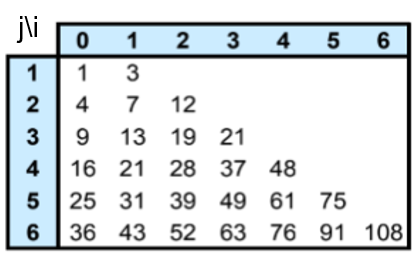
\includegraphics[width=0.4\textwidth]{imagenes/t22.png}
    \caption{Tabla de referencia.}
\end{figure}
\\ \\
Este método indica, que al tomar una célula de referencia se deberá desplazarse dos 
células en j y una en i. Por conveniencia se tomará la célula central como se muestra 
en la siguiente figura. Esto asegura que no exista un traslape en las frecuencias 
asignadas a los sectores de las células.
\begin{figure}[ht]
    \centering
    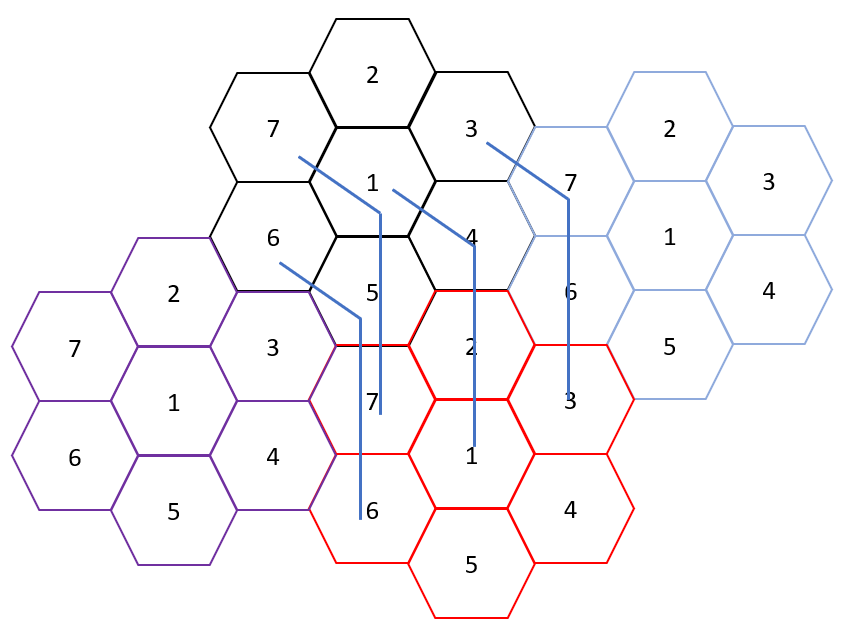
\includegraphics[width=0.7\textwidth]{imagenes/t23.png}
    \caption{Método i, j.}
\end{figure}
\\
Es importante señalar que el procedimiento que se muestra en la imagen anterior es 
ideal y no siempre se podrá seguir de manera exacta. Para el caso particular de este 
estudio, la distribución geográfica del municipio y la distribución de las zonas que 
no se deben radiar impiden aplicar este método al pie de la letra. Pero se sigue teniendo 
presente el objetivo de este método, que es el de evitar traslapes en la distribución de 
canales en los sectores de las células.

\subsection{Asignación de frecuencias}
La siguiente tabla muestra la asignación de frecuencias.
\begin{table}[ht]
    \centering
    \begin{tabular}{|l|l|l|l|l|}
    \hline
    Clúster & Célula & Sector & Número de canales & Canales \\ \hline
    1 & 1 & 1 & 95 & [1,31] \\ \hline
    1 & 1 & 2 &  & [32,63] \\ \hline
    1 & 1 & 3 &  & [64,95] \\ \hline

    1 & 2 & 1 & 95 & [96,127] \\ \hline
    1 & 2 & 2 &  & [128,159] \\ \hline
    1 & 2 & 3 &  & [160,191] \\ \hline

    1 & 3 & 1 & 95 & [192,287] \\ \hline

    1 & 4 & 1 & 95 & [288,383] \\ \hline

    1 & 5 & 1 & 95 & [384,431] \\ \hline
    1 & 5 & 2 &  & [432,479] \\ \hline

    1 & 6 & 1 & 95 & [480,527] \\ \hline
    1 & 6 & 2 &  & [528,575] \\ \hline

    1 & 7 & 1 & 95 & [576,623] \\ \hline
    1 & 7 & 2 &  & [624,671] \\ \hline

    2 & 1 & 1 & 95 & [1,31] \\ \hline
    2 & 1 & 2 &  & [32,63] \\ \hline
    2 & 1 & 3 &  & [64,95] \\ \hline

    2 & 2 & 1 & 95 & [96,191] \\ \hline

    2 & 3 & 1 & 95 & [192,223] \\ \hline
    2 & 3 & 2 &  & [224,255] \\ \hline
    2 & 3 & 3 &  & [256,287] \\ \hline

    2 & 4 & 1 & 95 & [288,335] \\ \hline
    2 & 4 & 2 &  & [336,383] \\ \hline

    2 & 5 & 1 & 95 & [384,431] \\ \hline
    2 & 5 & 2 &  & [432,479] \\ \hline

    2 & 6 & 1 & 95 & [480,575] \\ \hline
    \end{tabular}
    \caption{Distribución de canales.}
\end{table}

\newpage
\section{Análisis de áreas vulnerables}
El análisis de las áreas vulnerables se hará con fundamento en que deben de ser 
áreas no deben ser radiadas y no tengan cobertura indirecta de los sectores. Las 
áreas mas vulnerables que se analizaron son las siguientes. Los siguientes resultados también 
fueron calculados con la rutina anexada. 
\\ \\
\textbf{Clúster 1}
\\
Escuela Secundaría Oficial no. 219 Benjamín Hernández
\\
d=945.4m \quad $P_{Rx}$=-69.3dB
\\ \\
Escuela Secundaria FederalizadaTelpuchcalli
\\
d=945.4m \quad $P_{Rx}$=-75.9dB
\\ \\
Telesecundaria 10 Amado Nervo
\\ 
d=945.4m \quad $P_{Rx}$=-72.79dB
\\ \\
Escuela Telesecundaria Lic. José Vasconcelos
\\ 
d=945.4m \quad $P_{Rx}$=-70.65dB
\\ \\
Escuela Secundaria General Dr. Jaime Torres Bodet
\\ 
d=945.4m \quad $P_{Rx}$=-62.69dB
\\ \\
Escuela Secundaria Técnica 105 Calpulli
\\
d=945.4m \quad $P_{Rx}$=-66.93dB
\\ \\
Preparatoria Colegio de la Comunidad de Cd. Nezahualcóyotl
\\
d=945.4m \quad $P_{Rx}$=-70.3dB
\\ \\
\textbf{Clúster	2}
\\
Escuela Primaria Guadalupe Victoria
\\
d=945.4m \quad $P_{Rx}$=-64.79dB
\\ \\
Escuela Secundaria Técnica 9 Julián Carrillo
\\
d=945.4m \quad $P_{Rx}$=-74.13dB
\\ \\
Escuela Preparatoria Oficial No. 86.
\\
d=945.4m \quad $P_{Rx}$=-74.27dB
\\ \\
Reclusorio Femenil Tepozanes
\\
d=945.4m \quad $P_{Rx}$=-72.16dB
\\ \\
Cementerio Los Rosales
\\
d=945.4m \quad $P_{Rx}$=-82.26dB
\\ \\
Panteón Municipal \quad d=945.4m \quad $P_{Rx}$=-74.41dB
\\
Del análisis anterior se concluye que a pesar de ser zonas vulnerables, aun es posible 
tener una comunicación aceptable.

\section{Cálculos de eficiencia espectral y cantidad de llamadas}
Para la decada de los 80s y con el sistema AMPS, se propone un grado de servicio (GoS) de 
80\%.
\begin{equation}
    \frac{100-GoS}{100}=\frac{100-80}{100}=0.2
\end{equation}
Este valor es buscado en la tabla de Erlang A.
\begin{figure}[ht]
    \centering
    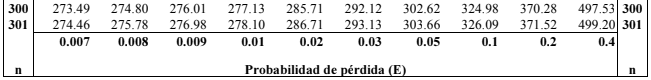
\includegraphics[width=0.99\textwidth]{imagenes/t24.png}
    \caption{Tabla Erlang A.}
\end{figure}
\\
Para los dos clústeres ($N_c$=2) que se tienen, hay un total de 1342 canales ($n_c$=1342).
\\ \\
Con estos valores se puede calcular el numero total de Erlangs para el numero de canales que se 
tienen.
\\ \\
$n=301 => A=371.52 \ Erlnag$
\\ \\
$n_c=1342->A_c=1656.411 \ Erlnag$
\\ \\
\begin{itemize}
    \item $BW_{CH}$: 30kHz = 0.03MHz.
    \item $BW_{Sis}$: 24MHz.
    \item Área: 46.74$km^2$.
\end{itemize}
Ahora sustituyendo los datos anteriores en las expresiones de la eficiencia espectral. 
\begin{equation}
    \eta=\frac{1}{BW_{CH}*N_C*Área}=\frac{1}{30*2*46.74}=356.582\mu[CH/MHz/km^2]
\end{equation}
\begin{equation}
    \eta=\frac{A \ Erlang}{BW_{Sis}*Área}=\frac{1656.411}{24*46.74}=1.476 [Erlang*MHz*km^2]
\end{equation}
Ahora se obtendrá el numero de llamadas con la siguiente expresión.
\begin{equation}
    A=\frac{N*\overline{t}}{h_p}
\end{equation}
Resolviendo para N.
\begin{equation}
    N=\frac{A*h_p}{\overline{t}}=\frac{1656.411*3600}{180}=33128.22 \ llamadas
\end{equation}
Con esta nueva información y recrodando el dato anterior del número de usuarios en la decada 
de los 80s, se obtiene la relacción de llamadas de 3min(180s) que puede hacer un usuario en 
una hora(3600s).
\begin{equation}
    \frac{N}{p(80s)}=\frac{61432}{33128}=1.854[\frac{llamadas}{usuarios}]
\end{equation}
Este número decimal puede indicarnos que un usuario puede empezar una segunda llamada, pero será 
liberada forzadamente después de un tiempo.

\section{Conclusión}
Revisando los resultados obtenidos se puede observar que el diseño propuesto no 
cumple los requerimientos para que los usuarios de la red realicen una llamada con 
éxito. Revisando el diseño de la red, se puede sugerir un mayor número de células 
más cerca entre sí. Es importante recordar que el municipio de Nezahualcóyotl es 
una de las regiones con mayor densidad poblacional del país. Se debe considerar 
este dato, ya que cada célula debe de dar servicio a un gran número de usuarios.

\newpage
\section{Anexo}
\subsection{Rutina}
\begin{lstlisting}[style=CStyle]
using System;
using System.Collections.Generic;
using System.Text;

namespace PotenciaRecepcion
{
    internal static class Program
    {
        public static void Main()
        {
            var potencias = new List<Potencia>
            {
                // Cluster 1 Celula 1
                new Potencia {NumeroCluster = 1, NumeroCelula = 1, NumeroSector = 1, Hb = 21, Hm = 1.7, D = 936.5, GtxDbi = 17.7, Gtx = 14.56, GrxDbi=9, Grx = 4.6, Ptx = 0.1, F = 900 },
                new Potencia {NumeroCluster = 1, NumeroCelula = 1, NumeroSector = 2, Hb = 20, Hm = 1.7, D = 930, GtxDbi = 17.7, Gtx = 14.56, GrxDbi=9, Grx = 4.6, Ptx = 0.1, F = 900 },
                new Potencia {NumeroCluster = 1, NumeroCelula = 1, NumeroSector = 3, Hb = 20, Hm = 1.7, D = 950, GtxDbi = 17.7, Gtx = 14.56, GrxDbi=9, Grx = 4.6, Ptx = 0.1, F = 900 },

                // Cluster 1 Celula 2
                new Potencia {NumeroCluster = 1, NumeroCelula = 2, NumeroSector = 1, Hb = 19, Hm = 1.7, D = 930, GtxDbi = 17.7, Gtx = 14.56, GrxDbi=9, Grx = 4.6, Ptx = 0.1, F = 900 },
                new Potencia {NumeroCluster = 1, NumeroCelula = 2, NumeroSector = 2, Hb = 19.5, Hm = 1.7, D = 940, GtxDbi = 17.7, Gtx = 14.56, GrxDbi=9, Grx = 4.6, Ptx = 0.1, F = 900 },
                new Potencia {NumeroCluster = 1, NumeroCelula = 2, NumeroSector = 3, Hb = 20, Hm = 1.7, D = 938, GtxDbi = 17.7, Gtx = 14.56, GrxDbi=9, Grx = 4.6, Ptx = 0.1, F = 900 },

                // Cluster 1 Celula 3
                new Potencia {NumeroCluster = 1, NumeroCelula = 3, NumeroSector = 1, Hb = 22, Hm = 1.7, D = 935, GtxDbi = 17.7, Gtx = 14.56, GrxDbi=9, Grx = 4.6, Ptx = 0.1, F = 900 },

                // Cluster 1 Celula 4
                new Potencia {NumeroCluster = 1, NumeroCelula = 4, NumeroSector = 1, Hb = 22, Hm = 1.7, D = 920, GtxDbi = 17.7, Gtx = 14.56, GrxDbi=9, Grx = 4.6, Ptx = 0.1, F = 900 },

                // Cluster 1 Celula 5
                new Potencia {NumeroCluster = 1, NumeroCelula = 5, NumeroSector = 1, Hb = 20, Hm = 1.7, D = 936, GtxDbi = 17.7, Gtx = 14.56, GrxDbi=9, Grx = 4.6, Ptx = 0.1, F = 900 },
                new Potencia {NumeroCluster = 1, NumeroCelula = 5, NumeroSector = 2, Hb = 19, Hm = 1.7, D = 938, GtxDbi = 17.7, Gtx = 14.56, GrxDbi=9, Grx = 4.6, Ptx = 0.1, F = 900 },

                // Cluster 1 Celula 6
                new Potencia {NumeroCluster = 1, NumeroCelula = 6, NumeroSector = 1, Hb = 19, Hm = 1.7, D = 940, GtxDbi = 17.7, Gtx = 14.56, GrxDbi=9, Grx = 4.6, Ptx = 0.1, F = 900 },
                new Potencia {NumeroCluster = 1, NumeroCelula = 6, NumeroSector = 2, Hb = 19.5, Hm = 1.7, D = 933, GtxDbi = 17.7, Gtx = 14.56, GrxDbi=9, Grx = 4.6, Ptx = 0.1, F = 900 },

                // Cluster 1 Celula 7
                new Potencia {NumeroCluster = 1, NumeroCelula = 7, NumeroSector = 1, Hb = 21, Hm = 1.7, D = 930, GtxDbi = 17.7, Gtx = 14.56, GrxDbi=9, Grx = 4.6, Ptx = 0.1, F = 900 },
                new Potencia {NumeroCluster = 1, NumeroCelula = 7, NumeroSector = 2, Hb = 20, Hm = 1.7, D = 935, GtxDbi = 17.7, Gtx = 14.56, GrxDbi=9, Grx = 4.6, Ptx = 0.1, F = 900 },

                // Cluster 2 Celula 1
                new Potencia {NumeroCluster = 2, NumeroCelula = 1, NumeroSector = 1, Hb = 19, Hm = 1.7, D = 937, GtxDbi = 17.7, Gtx = 14.56, GrxDbi=9, Grx = 4.6, Ptx = 0.1, F = 900 },
                new Potencia {NumeroCluster = 2, NumeroCelula = 1, NumeroSector = 2, Hb = 20, Hm = 1.7, D = 936, GtxDbi = 17.7, Gtx = 14.56, GrxDbi=9, Grx = 4.6, Ptx = 0.1, F = 900 },
                new Potencia {NumeroCluster = 2, NumeroCelula = 1, NumeroSector = 3, Hb = 22, Hm = 1.7, D = 938, GtxDbi = 17.7, Gtx = 14.56, GrxDbi=9, Grx = 4.6, Ptx = 0.1, F = 900 },

                // Cluster 2 Celula 2
                new Potencia {NumeroCluster = 2, NumeroCelula = 2, NumeroSector = 1, Hb = 24, Hm = 1.7, D = 940, GtxDbi = 17.7, Gtx = 14.56, GrxDbi=9, Grx = 4.6, Ptx = 0.1, F = 900 },

                // Cluster 2 Celula 3
                new Potencia {NumeroCluster = 2, NumeroCelula = 3, NumeroSector = 1, Hb = 25, Hm = 1.7, D = 936, GtxDbi = 17.7, Gtx = 14.56, GrxDbi=9, Grx = 4.6, Ptx = 0.1, F = 900 },
                new Potencia {NumeroCluster = 2, NumeroCelula = 3, NumeroSector = 2, Hb = 22, Hm = 1.7, D = 942, GtxDbi = 17.7, Gtx = 14.56, GrxDbi=9, Grx = 4.6, Ptx = 0.1, F = 900 },
                new Potencia {NumeroCluster = 2, NumeroCelula = 3, NumeroSector = 3, Hb = 21, Hm = 1.7, D = 950, GtxDbi = 17.7, Gtx = 14.56, GrxDbi=9, Grx = 4.6, Ptx = 0.1, F = 900 },

                // Cluster 2 Celula 4
                new Potencia {NumeroCluster = 2, NumeroCelula = 4, NumeroSector = 1, Hb = 19, Hm = 1.7, D = 937, GtxDbi = 17.7, Gtx = 14.56, GrxDbi=9, Grx = 4.6, Ptx = 0.1, F = 900 },
                new Potencia {NumeroCluster = 2, NumeroCelula = 4, NumeroSector = 2, Hb = 19.5, Hm = 1.7, D = 938, GtxDbi = 17.7, Gtx = 14.56, GrxDbi=9, Grx = 4.6, Ptx = 0.1, F = 900 },

                // Cluster 2 Celula 5
                new Potencia {NumeroCluster = 2, NumeroCelula = 5, NumeroSector = 1, Hb = 26, Hm = 1.7, D = 937, GtxDbi = 17.7, Gtx = 14.56, GrxDbi=9, Grx = 4.6, Ptx = 0.1, F = 900 },
                new Potencia {NumeroCluster = 2, NumeroCelula = 5, NumeroSector = 2, Hb = 25, Hm = 1.7, D = 936.5, GtxDbi = 17.7, Gtx = 14.56, GrxDbi=9, Grx = 4.6, Ptx = 0.1, F = 900 },

                // Cluster 2 Celula 6
                new Potencia {NumeroCluster = 2, NumeroCelula = 6, NumeroSector = 1, Hb = 20, Hm = 1.7, D = 940, GtxDbi = 17.7, Gtx = 14.56, GrxDbi=9, Grx = 4.6, Ptx = 0.1, F = 900 },
            };

            var vulnerables = new List<Potencia>
            {
                // Cluster 1 
                // Celula 1
                new Potencia {NumeroCluster = 1, NumeroCelula = 1, NumeroSector = 1, Hb = 21, Hm = 1.7, D = 945.4, GtxDbi = 17.7, Gtx = 14.56, GrxDbi=9, Grx = 4.6, Ptx = 0.1, F = 900 },

                // Celula 2
                new Potencia {NumeroCluster = 1, NumeroCelula = 1, NumeroSector = 1, Hb = 21, Hm = 1.7, D = 1370, GtxDbi = 17.7, Gtx = 14.56, GrxDbi=9, Grx = 4.6, Ptx = 0.1, F = 900 },

                // Celula 3
                new Potencia {NumeroCluster = 1, NumeroCelula = 1, NumeroSector = 1, Hb = 21, Hm = 1.7, D = 1150, GtxDbi = 17.7, Gtx = 14.56, GrxDbi=9, Grx = 4.6, Ptx = 0.1, F = 900 },

                // Celula 4
                new Potencia {NumeroCluster = 1, NumeroCelula = 1, NumeroSector = 1, Hb = 21, Hm = 1.7, D = 1020, GtxDbi = 17.7, Gtx = 14.56, GrxDbi=9, Grx = 4.6, Ptx = 0.1, F = 900 },

                // Celula 5
                new Potencia {NumeroCluster = 1, NumeroCelula = 1, NumeroSector = 1, Hb = 21, Hm = 1.7, D = 652.05, GtxDbi = 17.7, Gtx = 14.56, GrxDbi=9, Grx = 4.6, Ptx = 0.1, F = 900 },

                // Cluster 6
                new Potencia {NumeroCluster = 1, NumeroCelula = 1, NumeroSector = 1, Hb = 21, Hm = 1.7, D = 827.47, GtxDbi = 17.7, Gtx = 14.56, GrxDbi=9, Grx = 4.6, Ptx = 0.1, F = 900 },

                // Celula 7
                new Potencia {NumeroCluster = 1, NumeroCelula = 1, NumeroSector = 1, Hb = 21, Hm = 1.7, D = 1000, GtxDbi = 17.7, Gtx = 14.56, GrxDbi=9, Grx = 4.6, Ptx = 0.1, F = 900 },

                // Cluster 2
                // Celula 1
                new Potencia {NumeroCluster = 1, NumeroCelula = 1, NumeroSector = 1, Hb = 21, Hm = 1.7, D = 733.64, GtxDbi = 17.7, Gtx = 14.56, GrxDbi=9, Grx = 4.6, Ptx = 0.1, F = 900 },

                // Celula 2
                new Potencia {NumeroCluster = 1, NumeroCelula = 1, NumeroSector = 1, Hb = 21, Hm = 1.7, D = 1240, GtxDbi = 17.7, Gtx = 14.56, GrxDbi=9, Grx = 4.6, Ptx = 0.1, F = 900 },

                // Celula 3
                new Potencia {NumeroCluster = 1, NumeroCelula = 1, NumeroSector = 1, Hb = 21, Hm = 1.7, D = 1250, GtxDbi = 17.7, Gtx = 14.56, GrxDbi=9, Grx = 4.6, Ptx = 0.1, F = 900 },

                // Celula 4
                new Potencia {NumeroCluster = 1, NumeroCelula = 1, NumeroSector = 1, Hb = 21, Hm = 1.7, D = 1110, GtxDbi = 17.7, Gtx = 14.56, GrxDbi=9, Grx = 4.6, Ptx = 0.1, F = 900 },

                // Celula 5
                new Potencia {NumeroCluster = 1, NumeroCelula = 1, NumeroSector = 1, Hb = 21, Hm = 1.7, D = 1960, GtxDbi = 17.7, Gtx = 14.56, GrxDbi=9, Grx = 4.6, Ptx = 0.1, F = 900 },

                // Cluster 6
                new Potencia {NumeroCluster = 1, NumeroCelula = 1, NumeroSector = 1, Hb = 21, Hm = 1.7, D = 1260, GtxDbi = 17.7, Gtx = 14.56, GrxDbi=9, Grx = 4.6, Ptx = 0.1, F = 900 },
            };

            var reglones = new StringBuilder();
            var vulnerable = new StringBuilder();

            foreach (var potencia in potencias)
            {
                var lo = Math.Round((32.4 + 20 * Math.Log10(potencia.F) + 20 * Math.Log10(potencia.D / 1000)), 2);
                var prx = Math.Pow((potencia.Hb * potencia.Hm) / Math.Pow(potencia.D, 2), 2) *
                               ((potencia.Gtx * potencia.Grx) / lo) * potencia.Ptx;
                potencia.Prx = 10 * Math.Log10(prx / 0.001);

                reglones.Append($"{potencia.NumeroCluster} & {potencia.NumeroCelula} & {potencia.NumeroSector} & " +
                                $"{potencia.Hb} & {potencia.D} & {potencia.Gtx} & {potencia.Grx} & " +
                                $"{lo} & {Math.Round(potencia.Prx, 2)} \\\\ \\hline" + Environment.NewLine);
            }

            foreach (var potencia in vulnerables)
            {
                var lo = Math.Round((32.4 + 20 * Math.Log10(potencia.F) + 20 * Math.Log10(potencia.D / 1000)), 2);
                var prx = Math.Pow((potencia.Hb * potencia.Hm) / Math.Pow(potencia.D, 2), 2) *
                          ((potencia.Gtx * potencia.Grx) / lo) * potencia.Ptx;
                potencia.Prx = 10 * Math.Log10(prx / 0.001);

                vulnerable.Append($"{potencia.NumeroCluster} & {potencia.NumeroCelula} & {potencia.NumeroSector} & " +
                                $"{potencia.Hb} & {potencia.D} & {potencia.Gtx} & {potencia.Grx} & " +
                                $"{lo} & {Math.Round(potencia.Prx, 2)} \\\\ \\hline" + Environment.NewLine);
            }


            var rows = reglones.ToString();
            var rows2 = vulnerable.ToString();
        }

        private class Potencia
        {
            public double Hb { get; set; }
            public double Hm { get; set; }
            public double D { get; set; }
            public double GtxDbi { get; set; }
            public double Gtx { get; set; }
            public double GrxDbi { get; set; }
            public double Grx { get; set; }
            public double Ptx { get; set; }
            public double F { get; set; }
            public double Prx { get; set; }

            public int NumeroCluster { get; set; }
            public int NumeroCelula { get; set; }
            public int NumeroSector { get; set; }
        }
    }
}

\end{lstlisting}

\newpage
\subsection{Mapa}

\end{document}